% latex file for generating the development notes

\documentclass{article}

\usepackage{cite}% Make references as [1-4], not [1,2,3,4]
\usepackage{url}  % Formatting web addresses 
\usepackage{amsmath}
\usepackage{amssymb}
\usepackage{epsfig}


% Article top matter
\title{yeast\_MFC Developer Notes} %\LaTeX is a macro for printing the Latex logo
\author{Ryan Tasseff, \texttt{rtasseff@systemsbiolgy.org}}  %\texttt formats the text to a typewriter style font
\date{\today}  %\today is replaced with the current date



\begin{document}

\maketitle


\begin{abstract}
Detailed notes of the development of the yeast microfludic chip model,
using the Biocellion framework.
The model will capture the behavior of 
budding yeast and the surrounding environment in a chip designed 
designed to trap single yeast cells for time laps imaging.
Here we track the development of the model over time.
A loose organizational scheme is used, with components then function then time.
The document is dynamic will will change and the project progresses. \end{abstract}
 
\section{Introduction}
Here we will cover the development of the yeast microfludic chip model,
using the Biocellion framework.
The primary goal of the model is to capture the behavior of 
budding yeast and the surrounding environment in a chip  
designed to trap single yeast cells for time laps imaging.
Specifically, we wish to model simple aspect of yeast: 
movement, budding/ division, death and nutrient uptake.
We also want to capture the diffusion and (if needed) the 
convection/ advection of key molecules, 
to model there spatial distribution over time.

The following is a rough guide to how the model was/ is being developed.
There is no specific structure; however, 
we will attempt to organize first by specific model components, 
then by relevant biology/ function and finally by date (time stamp on all additions).
To some extent, we will leave deprecated code/ descriptions
in the notes; however, we will try to mark them as deprecated.

\section{General Assumptions, Simplifications and Implementation Details}
\subsection{Units}
time = seconds (sec);
length = micrometers ($\mu m$);
volume = cubic micrometers ($\mu m^3$);
mass = micro grams ($\mu g$);
concentration = $frac\{\mu g}{\mu m^3}$;

\subsection{Growth and Division}
\emph{20131111} We are assuming a simple model of growth, division and cell cycle control\cite{Charvin2009}.
The primary assumptions are 1) exponential growth of cells
2) perfect volume control,
the cells do not start a clock until some $V_C$ is reached;
2b) all additional volume will be transfered to daughter;
3) linear progression through cell cycle;
3b) completely deterministic mitosis, 
the cell finishes division after clock hits 1.
Currently, we have added some additional simplification and assumptions:
1) cells do not bud they just grow and divide end of cycle,
this will be improved by forming a junction with m and d cells after g1, 
which will break after cycle ends,
unfortunately it may be trick to implement exp vol increase in d based on m vol;
2) budding is always at same spot so we will track it,
unfortunately this will not do much until we implement rotation

\subsection{Physical Environment}
\emph{20131111} Although the model does contain 3 dimensions,
we will focus only on the first 2 (x,y), 
and assume movement is restricted in z-axis based on chip size.
This assumption should be naturally enforced if we make no movement in z-axis.
\textbf{NOTE:} This obviously will not account for any forces due to the z-axis,
for example making the width smaller will not increase friction and will not effect particle movement at all.
\emph{20131112} Because we will be using a complex shape we will have to define special regions.
Currently regions can be defined as uninhabitable, and no agents will be allowed in, and
as PDE and pde diffusion at interface will be manually set to zero.
\textbf{NOTE:} While PDE buffer MAY be enough to constrain molecules we will need more with agents.
We should find a way to see if the box is uninhabitable, 
implement shoving and perhaps even friction and rotational forces.

The shape of the trial system will be modeled after figure \ref{FIG:chip}.
The x-axis will be along the horizontal, 
which is perpendicular to the flow channel.
The chip is modeled at the scale of a unitbox (close to the size of a single cell).
The unitbox will be defined as open (1) or closed (0) via a desing matrix,
and this will be used to setup habitability, diffusion and other constants.
therefore, the x-boundary conditions for diffusive molecules will be Dirchlet.
They will be set to maintain the same concentration in the channel itself.
Other boundaries will be Numman assuming no flux through walls.

\subsection{Nutrient Constraints}
\label{S:nutriant}
\emph{20131111} We will assume that nutrients is required for growth and division.
Currently we treat glucose as only required nutrient.
We assume uptake is constant.
Estimates were provided by Gilles Lab to be an uptake of
$2.5E-12 \frac{g}{min*cell}$ which comes out to 4.2E-5 $\frac{ng}{sec*cell}$.
The bulk concentration in the flow channel is $20\frac{g}{L}$ which comes to 2E-2 $frac\{ng}{\mu m^3}$.



\subsection{Mechanical Forces and Interactions}
Currently, as mentioned above, 
we have NO interactions with the walls at this moment,
except for the fact the disp is recalculated to prevent penetration.
Only agent agent shoving produces force.
Displacement will be calculated based on an overdamped system:
\begin{equation}
\dot{x} = \frac{1}{c} \sum F
\label{EQ:disp}
\end{equation}
where $c$ is the friction coefficient and $F$ is the force, the dot denotes change with respect to time.
Here a simple finite difference model is used to calculate delta x.
   

 


\section{Initialization}
\emph{20130927} We have initialized the model using the PDE example provided in Biocellion.

\section{Model Properties and Definitions}
The following is a general overview of the various elements on the model.
Nearly all is defined in model \textit{model\_define.h}.

\subsection{Agent types and properties}
\emph{20130927} We will add agents under `---Agents---'.
The primary agent is \texttt{AGENT\_YEAST\_CELL}.
We also added the initial properties in the same place,
specifically we have added 2 model reals that describe the 
location of the budding direction \texttt{YEAST\_CELL\_MODEL\_REAL\_BUD\_DIR\_}.
\emph{20130927} The property \texttt{YEAST\_CELL\_MODEL\_REAL\_CC\_CLOCK}
was added to monitor progression through the cell cycle \cite{Charvin2009}
Additional cell properties added under `---Cell Properties--- including 
`-Growth and Division-' properties taken from \cite{Charvin2009} to describe the cell cycle.

Uptake of diffusible elements is also possible,
Standard constant values are being used for this first impl using \texttt{.
Currently we have only one element so its a real, 
but we should change to array if more are added.
This would be reflected under `---Difusable elements---'.
Estimate was provided as above in \ref{S:nutriant}.
As for diffusion we are assuming a constant, except at boundaries,
and assuming the solvent is water.
The diffusion coef for glucose was found to be 600 $\frac{\mu m^2}{sec}$,
found in bionumbers.hms.harvard.edu.



\subsection{Grid Properties} 
Props found under `---Grid Properties---'.

The flow channel is modeled by constant concentration boundary conditions, 
these are set in \texttt{ELEM\_BULK\_CONCENTRATION}.
Currently we have only one element so its a real, 
but we should change to array if more are added.
This would be reflected under `---Difusable elements---'.
Estimate was provided as above in \ref{S:nutriant}. 


\subsection{Domain}
\emph{20131113} Under `---Domain---'
Unit box size \texttt{IF\_GRID\_SPACING} is set to maximum interaction dist 
\texttt{CELL\_INTRCT\_DIST\_MAX} which is the cell diameter of the largest cell.
Currently we assume that the largest cell is double the critical volume,
and critical volume corresponds to a sphere with 2 $\mu$m radius (estimate).
\textbf{NOTE:} Once budding is introduced cells will not grow very large before division,
and we can reduce the maximum size and the grid spaces will also reduce.

Design of the domain is given by \texttt{CHIP\_DESIGN\_MATRIX}, 
entries are zero and one.




\section{Agent Rules}
Rules defined in \textit{model\_routine\_agent.cpp} unless otherwise stated.

\subsection{updateSpAgent}
\emph{20131111} We define growth here.  
Currently, we have deterministic exponential volume increase.
Which is achieved by simple steps.  
\emph{20131113} Moved cell cycle to here to connect with uptake.
Here have track movement through the cell cycle by linearly increasing the phase variable under ` ---Cell Cycle Progression---'.
Both growth and cell cycle progression only occur if enough glucose is available.
We calculate the total amount of nutrients in the box and the needs,
if enough is present we set a model real, \texttt{YEAST\_CELL\_MODEL\_REAL\_ELEM\_GLUCOSE\_UPTAKE},
to the amount we expect to take for this step and we allow growth and clock to update.



\subsection{updateSpAgentBirthDeath }
\emph{20131111} We are doing all division at a single step,
as opposed to a bud.
So when cell cycle is complete we allow the cells to divide.
Based on \cite{Charvin2009} cell cycle is complete after the clock reaches 1.0.
The limit is defined in \textit{model\_define.h} as \texttt{CC\_CLOCK\_CRITICAL}.
We note that the phase is tracked as an internal variable \texttt{YEAST\_CELL\_MODEL\_REAL\_CC\_CLOCK}

\subsection{adjustSpAgentState}
\emph{20131111} Very simple model to calculate velocity based on EQ \ref{EQ:disp}.
Finite difference gets us from velocity to displacement.
Added under `---DISP---'.

\subsection{divideSpAgent}
\emph{20131111} Division is done all at once.  
After the cell cycle is complete this method will be called.
All volume above the critical volume is sent to the daughter.
Displacement is done so that both move to account for new radius, 
and this is in the direction of the budding, defined as a property in \textit{model\_define.h}.
 

\section{Mechanical Interactions}
Rules defined in \textit{model\_routine\_mech\_intrct.cpp} unless otherwise stated.

\emph{20131112} Standard force will be calculated based on shoving only.
Shoving is basically like the positive potnetail part of the spring potential,
The spring constant is the cell stiffness \texttt{CELL\_STIFF}, 
which defined in \textit{model\_define.h} and set to allow 50\% of total disp from shoving.





\begin{figure}
\begin{center}
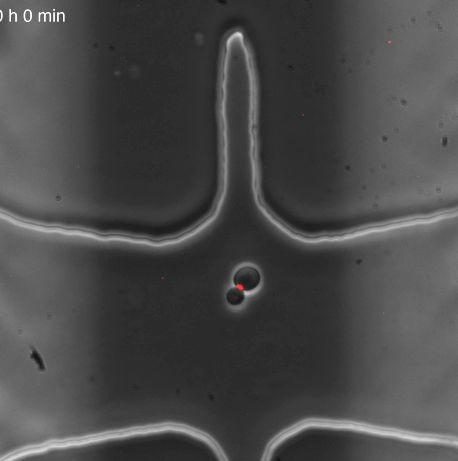
\includegraphics{figs/chip.png}
\caption{Screen shot of loaded chip.  
Flow channels are on the left and right (out of frame).
The model will simulate x-axis along or parallel to the horizontal of this image, 
and y-axis along or parallel to the vertical.}
\label{FIG:chip}
\end{center}
\end{figure}







\bibliographystyle{plain}
\bibliography{mainRefDB}

\end{document}  %End of document.
